\documentclass[10pt,twocolumn,letterpaper]{article}

%%%%%%%%% PAPER TYPE  - PLEASE UPDATE FOR FINAL VERSION
% \usepackage[review]{cvpr}      % To produce the REVIEW version
% \usepackage{cvpr}              % To produce the CAMERA-READY version
\usepackage[pagenumbers]{cvpr} % To force page numbers, e.g. for an arXiv version

% Include other packages here, before hyperref.
\usepackage{graphicx}
\usepackage{amsmath}
\usepackage{amssymb}
\usepackage{booktabs}
\usepackage{tablefootnote}
\usepackage{booktabs}
\graphicspath{{"../results/"}}

% It is strongly recommended to use hyperref, especially for the review version.
% hyperref with option pagebackref eases the reviewers' job.
% Please disable hyperref *only* if you encounter grave issues, e.g. with the
% file validation for the camera-ready version.
%
% If you comment hyperref and then uncomment it, you should delete
% ReviewTempalte.aux before re-running LaTeX.
% (Or just hit 'q' on the first LaTeX run, let it finish, and you
%  should be clear).
\usepackage[pagebackref,breaklinks,colorlinks]{hyperref}


% Support for easy cross-referencing
\usepackage[capitalize]{cleveref}
\crefname{section}{Sec.}{Secs.}
\Crefname{section}{Section}{Sections}
\Crefname{table}{Table}{Tables}
\crefname{table}{Tab.}{Tabs.}


%%%%%%%%% PAPER ID  - PLEASE UPDATE
\def\cvprPaperID{*****} % *** Enter the CVPR Paper ID here
\def\confName{CVPR}
\def\confYear{2022}


\begin{document}

%%%%%%%%% TITLE - PLEASE UPDATE
\title{Transfer learning models for tree species detection in agroforestry}

\author{Erich Trieschman\\
Stanford University, Department of Statistics\\
{\tt\small etriesch@stanford.edu}
% \and
% Second Author\\
% Institution2\\
% First line of institution2 address\\
% {\tt\small secondauthor@i2.org}
}
\maketitle

%%%%%%%%% ABSTRACT
\begin{abstract}
  Tree species identification can integrate with a broader suite of tools to improve the accuracty of forest carbon estimation while also reducing costs. In this paper I train a tree species classifier to support carbon measurements in the agroforestry setting. I compile a novel dataset of over 24k labeled tree images and evaluate six transfer learning models for highest performance. 
  
  My dataset is constructed predominantly from scraped image searches for each tree species through the Microsoft Bing search engine. I pair this dataset with scraped images of several other tree databases as well. My dataset is augmented with vertical reflections and random croppings of each image and finally filtered with a binary classification model trained to detect trees.
  
  I achieve a Top-1 accuracy of [[XX]] on held-out data by applying transfer learning to the [[XX]] model, training the entire last convolutional block of the model. I find this model to be better optimized for mobile-based tree species identification than other models because of its lower model parameter count. I find this final model performs best at detecting [[TREESPECIES]] with a precision and recall of XXX, respectively; it performs least well at detecting [[TREESPECIES]] with a precision and recall of XXX respectively.
\end{abstract}

%%%%%%%%% BODY TEXT
\section{Introduction}
\label{sec:intro}
Trees are a large carbon pool for our planet. They play a vital role in offseting anthropogenic carbon emissions and attenuating the effects of climate change. We can grow this pool through afforestation and deferred deforestation, oftentimes supported through carbon offset payments by sectors emitting carbon to the landowners growing these forests. 

One high-potential opportunity for afforestation is through the transition of pastureland operations to silvopasture operations. Silvopasture is simply the agricultural practice of combining tree cropping with livestock management. 

In order for a payment system like this to work, we need a highly accurate estimate of the amount of carbon stored in trees. Fortunately, decades of research has been invested into tree growth projections and today, allometric equations are readily available for many tree species, which can accurately estimate above and below-ground tree biomass as a function of tree height, tree diameter, species, and local climate. 

This research develops a novel dataset of tree photographs and trains a deep learning model to identify tree species from images in the silvopasture setting. These tools will be combined with a broader suite of tools being developed to accurately estimate tree carbon from phone-based tree height and diameter measurements to enable carbon payments on agricultural operations transitioning to silvopasture. In the future, these phone-based measurements will be used to augment and improve the models developed in this paper.

Specifically, in this paper I compile a novel dataset of high-fidelity tree photographs, taken in profile perspective. The dataset contains classified images of the 7 most common tree species used in silvopasture in the southeastern US, where pilot projects for this silvopasture transition are underway. I then train a deep learning model to predict tree species from these profile-vew tree photographs.

%------------------------------------------------------------------------
\section{Related work}
\label{sec:litreview}

Image classification is a common problem solved using convolutional neural networks. Beginning in late 2012, we have experienced step changes in the performance of neural networks for image classification first with the introduction of AlexNet and later with further improvements through neural net models like VGGNet, ResNet, and GoogLeNet \cite{VGGNet, GoogLeNET, ResNET}. These latter models each incremented the field with refinements to parallelization and the ability to exploit backpropagation into deeper and deeper networks.

Within this time period there has been a plethora of work focused on image classification, from general problems to more specific, with only limited research focused on profile-perspective tree species identification. Below I summarize some of the research focused on this problem and the methods that support it. 

In Feng et al.'s work on long-tailed object detection, the team explores training classification models on highly-similar objects, a similar challenge to that conducted in this paper \cite{Feng_2021_ICCV}. Feng et al. achieve increased performance via an Equilibrium Loss (EBL) and a Memory-augmented Feature Sampling (MFS) method, improving detection performance.

Carpentier et al. use a self-collected dataset to solve a very similar classification problem to my own: tree detection through bark images \cite{Carpentier_2018}. The team trains deep neural network models for this classification task and achieves an accuracy of over 90\% in predicting tree species for over 23 different species of trees and tree diameters. Interestingly, the team finds that increasing the number of individual trees in the training database is one of the most important factors to achieving a high accuracy score.

Fricker et al. also attempts to classify trees, however from an aerial perspective instead of the profile perspective taken in this paper \cite{Fricker_RS_2019}. The team uses field-based training data, high spatial resolution airborne hyperspectral imagery, and a convolutional neural network classifier to train a model for future detection using lower-cost input data. Fricker finds significant improvements in the accuracy of his model when using hyperspectral data over simple RGB. 

%------------------------------------------------------------------------
\section{Methods}
\label{sec:methods}
The objective of this paper is to develop a model with highest Top-1 accuracy (lowest Top-1 misclassification error) for the identification of tree species from tree photographs, while also balancing the size of the model. These metrics best align with the downstream use case of the model, which is to assist in the proper identification of agroforestry trees through a mobile-based app. 

To achieve a model with highest Top-1 accuracy, I construct several shallow baseline models and several deep transfer-learning models (see Subsection \ref{sec:models}). I train all models on a training subset of my novel tree photograph dataset and use a validation subset of this dataset to evaluate the performance of my trained models (see Subsection \ref{sec:model_sel}). Finally, I use a test subset of this dataset to determine the final performance metrics of my selected model (see Results section below).  

\subsection{Model construction}
\label{sec:models}
I evaluate four baseline classificaiton models in this report. These models serve as a standard against which I can aim to improve Top-1 accuracy through the use of deep convolutional neural networks. I implement the remaining models in this research through a transfer learning approach, where I leverage pretrained model weights of existing, high-performing image classification models, and focus only on relearning the outermost layers of the model, trained specifically to my novel dataset.

I provide a summary of these models in Table \ref{tab:model_desc} and describe them in more detail in the sections below.

\begin{table}[!htbp]
  \begin{center}
    \small
  \begin{tabular}{|l|l|l|l|}
  \hline
  Model & Loss & Layers/Vers. & Transf. learn.\\
  \hline\hline
  Softmax & CrossEnt & 1 & False \\
  SVM & Hinge & 1 & False \\
  FCN & CrossEnt & 2 & False \\
  CNN & CrossEnt & 3 & False \\
  ResNet & CrossEnt & 50 & True \\
  ConvNext & CrossEnt & ``Tiny'' & True \\
  Transformer & CrossEnt & 12: 16x16pix & True \\
  \hline
  \end{tabular}
  \end{center}
  \caption{\label{tab:model_desc} Summary of evaluated models}
  \end{table}

\subsubsection{Baseline models}
The models I consider are a multiclass softmax model, a multiclass support vector machine model (SVM), a two-layer fully connected network (FCN), and a 3-layer convolutional network (CNN). The softmax and SVM models serve as the highest-level attempts at class identification, while the FCN was meant to reveal potential gains from including non-linear activation functions, and the CNN to reveal potential gains from capturing image structure. I construct all models with Pytorch's "nn.Sequential" module \cite{PyTorch}.

To construct the softmax model, I first flatten my images, removing all spatial structure, then transform the output to a 7-class dimension with learnable weights. I then use a softmax activation function paired with the negative log likelihood loss function. Together, these are equivalent to the cross entropy loss function, which I use in all but the SVM model. The cross entropy loss function is given by
\begin{align}
  \mathcal{L} = \{l_1, \dots, l_N\}^T, l_i = \log\frac{\exp{x_{i, y_i}}}{\sum_{c=1}^C\exp{x_{i,c}}}
\end{align}
Where $s_{y_i}$ is the score for the correct class. 
To construct the SVM model, I flatten my images, transform the output to a 7-class dimension with learnable weights, and train my model using the multi-margin loss function given by
\begin{align}
  \mathcal{L} = \{l_1, \dots, l_N\}^T, l_i = \sum_{i=1, i\neq y}^N \max(0, x_{i} - x_{y_i} + 1)
\end{align}
To construct the FCN model, I flatten my images and define a single hidden layer of dimension 500 with a ReLU activation function, I then transform the output to a 7-class dimension with learnable weights. To construct the CNN model, I preserve the structure of my images and pass them through two convolutions, the first with kernel size of 5 and 32 channels, and next with kernel size of 3 and 16 channels. Both layers use a ReLU activation function and I pad images so that the output image shape is preserved throughout the model. Finally I flatten the structured data and transform the output to a 7-class dimension with learnable weights. 

\subsubsection{Transfer learning models}
The first transfer learning model I consider is a deep convolutional neural network with residual connections (ResNet) introduced by He at al. \cite{ResNET}. The original model has 152 layers and relies on a residual learning layers which are easier to train and optimize than conventional feed-forward layers used in my baseline modeling section. This residual learning framework addresses degrading training accuracy in deeper networks by incorporating residual mappings between sets of convolutional layers. Although the original architecture consists of 152 layers, smaller versions of the same network are also available; I choose ResNet-50 because it significantly reduces the number of parameters and may offer faster operation performance on mobile devices. 

The next transfer learning model I consider is a vision transformer (ViT) introduced by Dosovitskiy et al. \cite{ViT}. The original model has 32 layers and 16x16 pixel input patches and relies entirely on attention modules that process smaller, 2D patches of the image, and demonstrating that models without convolutional layers can perform as well or better than models with them. This framework also requires substantially fewer resources to train than a convolutional neural network and can accelerate training times and reduce training computation and economic costs. Smaller versions of the same network are also available. I choose the 12-layer 16x16 pixel input patch model because it significantly reduces the number of parameters and may offer a faster operation performance on mobileprediction performance on mobile devices.

The final transfer learning model I consider is a modernized convolutional network with residual features (ConvNeXt) introduced by Liu et al. \cite{ConvNext}. The original model is based on the original ResNet-152 model, but reevaluated at macro and micro levels for similarities and differences with modern-day vision transformers. This framework is meant to provide a high-performing convolutional framework with equal performance to vision transformers. Smaller versions of the same network are also available. I choose the "tiny" version because it significantly reduces the number of parameters and may offer a faster operation performance on mod prediction performance on mobile devices.

I use the PyTorch pretrained model implementations of ResNet, ConvNeXt, and ViT, available through its "models" module \cite{PyTorch}. In each transfer learning model, I substitute the last fully connected layer with a two-layer fully connected network. I use a hidden layer dimension of 128 and a ReLU activation function in all transfer learning models. The final output layer output is of size 7, the number of species in my target tree-classification model. 

\subsection{Model training}
\label{sec:model_sel}
In this section I describe my model training process and the set-up for my model selection.
I begin by randomly splitting my dataset (described in more detail in Section \ref{sec:data}) into train, validation, and test datasets. I withold 10\% of my data (2,789 images) for final evaluation of my selected model (see Section \ref{sec:results}). Out of the remaining dataset, I use 25\% (6,274 images) for validation and 75\% (18,819 images) for training.
I train all models described above in minibatches of 32 images. I use stochastic gradient descent with Nesterov momentum of 0.9 as my optimization algorithm. Stochastic gradient descent computes gradients on batches of training data and performs gradient updates on all weights with those batch-computed gradients. Including Nesterov momentum provides a technique for computing this gradient descent at a point "ahead" of the current location of the weights, which can greatly accelerate convergence \cite{nesterov}. The equations for SGD with a Nesterov accelerated gradient follow
\begin{align*}
  v_t &= \mu_{t-1}v_{t-1} - \epsilon_{t-1}\nabla f(\theta_{t-1} + \mu_{t-1}v_{t-1})\\
  \theta_t &= \theta_{t-1} + v_t
\end{align*}
Where $\theta_t$ are the model parameters, $v_t$ the velocity, $\mu_t \in [0,1]$ momentum (decay) coefficient (0.9 in my case) and $\epsilon_t > 0$ the learning rate at iteration t, $f(\theta)$ is the objective function and $\nabla f(\theta)$ the gradient.
I train all baseline models with a learning rate that starts at 0.0001 and decays every two epochs by a factor of 10. I train all baseline models for four epochs and all transfer learning models for 6 epochs.
Last to mention, I train all three transfer learning models under two regimes. First, I freeze the weights of all but the final, additional two-layer fully connected hidden network I add to the training models. In this regime, only this final two-layer network is trained on all images and I leverage the existing weights of the pretrained models for all other layers. 
Second, I freeze the weights of all but the final convolutional or decoder block in each transfer learning model. For ResNet I train the fourth and final convolutional block, for ConvNeXt I retrain the 25th convolutional network block, and for ViT I retrain the 11th encoder module.

%------------------------------------------------------------------------
\section{Dataset and features}
\label{sec:data}
This paper develops a novel dataset of high-fidelity tree photographs, taken in profile perspective, labeled with the tree species. The species included are the seven most common species of tree used in silvopasture in the southeastern US: Black Locust, Black Walnut, Honey Locust, Loblolly Pine, Northern Red Oak, Pecan, Chinese Chestnut. 

I compile these photographs and labels from images scraped from the internet. I augment augment my dataset with reflections and random scaled croppings of each image. All original and tranformed images are then center-cropped and scaled for use in a deep learning model. Lastly, the dataset is filtered using a binary classifier trained to identify profile images of trees to ensure that the image dataset scraped from the internet has a high likelihood of only containing trees. I provide sample images from this dataset with their tree likelihood in Figure \ref{fig:samp_imgs} and I provide full detail of how this novel dataset is constructed in the subsections below.

\begin{figure}[!htbp]
  \centering
  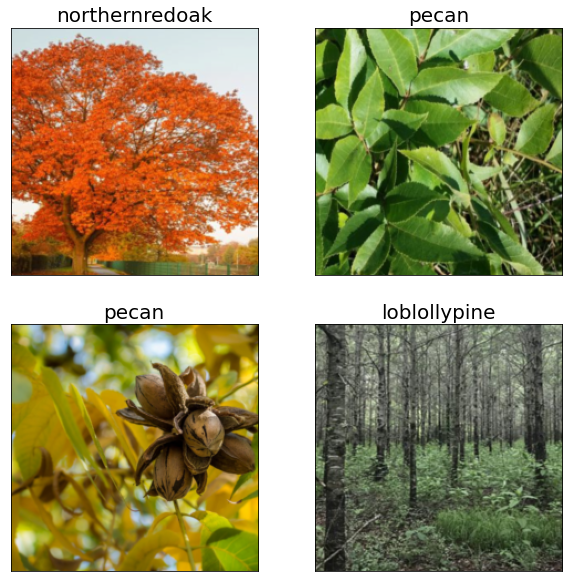
\includegraphics[width=.8\linewidth]{"./fig_samp_imgs.png"}
  \caption{\label{fig:samp_imgs} Sample images from final dataset}
\end{figure}

%-------------------------------------------------------------------------
\subsection{Image scraping}

I use three data sources to generate a dataset of tree images: the Harvard Arboretum Plant Image database \cite{harvard}, the Arbor Day Foundation website \cite{arborday}, and the results of Microsoft Bing image searches for each tree species of interest. I also evaluated BarkNet, a dataset of close-up photographs of tree bark supporting a tree-bark identification model, however, this dataset did not contain any of the species of interest in this project.

I developed website-specific python codes to scrape and download images of each tree species from each source. I downloaded all available images from the Harvard Arboretum and Arbor Day sources for each of the species of interest. And for the results of my Bing Image searches, I downloaded all of the first 750 images that were not protected from download access. I use Bing image search instead of Google image search because of recent changes in Google's website layout that make web scraping more difficult.

This results in a preliminary dataset of 7,707 images, detailed in Table \ref{tab:dataset_og}.

\begin{table}[!htbp]
   \begin{center}
    \small
   \begin{tabular}{|l|r|r|r|r|}
   \hline
   Species (N) & Total & Bing & Arb. Day & Harvard \\
   \hline\hline
   Black Locust & 605 & 562 & 0 & 43\\
    Black Walnut & 651 & 563 & 4 & 84\\
    Honey Locust & 501 & 501 & 0 & 0\\
    Loblolly Pine & 495 & 488 & 7 & 0\\
    North. Red Oak & 579 & 531 & 7 & 41\\
    Pecan & 611 & 591 & 6 & 14\\
    Chinese Chestnut & 662 & 467 & 3 &  192\\
    \hline\hline
    Total & 7707 & 6905 & 54 & 748\\
   \hline
   \end{tabular}
   \end{center}
   \caption{\label{tab:dataset_og} Number of images, by data source and species}
   \end{table}

%-------------------------------------------------------------------------
\subsection{Dataset augmentation}

I augment the dataset with a reflection of each image about its vertical axis. I do not include horizontal and diagonal reflections because all tree images classified with this model are expected to be up-right. I also augment the dataset with the original and mirror image of a random cropping of each image at 3 different relative sizes: 10\%, 25\%, and 50\%. 

In total, this augmentation increases my dataset by a factor of eight and results in a dataset of 32,832 images.

%-------------------------------------------------------------------------
\subsection{Image cropping, scaling, and }

I center and scale all images to the same shape and size for use in a deep learning model. I first upscale all images so that the minimum dimension of each image (height or width) is 1024 pixels. I next center-crop each image to a 1024x1024 pixel square. And finally I downscale all images to 224x224 pixels and normalize them based on the mean and standard deviation of the datset used by Pytorch developers to pretrain their available models \footnote{RGB means = [0.485, 0.456, 0.406]; RGB standard deviations = [0.229, 0.224, 0.225]}. These transformations are implemented so that this image dataset follows the common dimensions and normalizations used by the pretrained models available for use through Pytorch \cite{PyTorch}. 

%-------------------------------------------------------------------------
\subsection{Dataset filtering}

Lastly, I filter my dataset to only include, with high likelihood, profile-perspective photographs of trees. I choose to filter my dataset because the method I use to construct my dataset introduces erroneous images with somewhat high likelihood. I confirmed this with manual inspection, observing errors like drawings of trees or images loosely related to trees (e.g., a table made from the wood of a black walnut tree). The former is more of a concern in the Harvard Arboretum and Arbor Day Foundation datasets, and both the former and latter are concerns in the results of Bing image searches. My dataset also includes random croppings of all images, which may not include any component of a tree and I choose to filter these croppings too.

There are no publicly available binary classification models for tree images, so I use transfer learning to leverage the pretrained weights of ResNet50 and construct a binary classifier \cite{ResNET} specific to this research. I do so by replacing the final fully connected layer of ResNet50 with the same fully connected layers and pooling described in the methods section above.

To train these final layers of the pretrained ResNET model, I create a separate dataset of tree and not-tree images, labeled as such, by scraping Bing for select search terms. I include images of "tree photograph", "tree bark photograph", and "tree leaf photograph" in the tree class, and I include images of "tree drawing", "table", "hand", "map", and "diagram" in the not-tree class; I determined this not-tree search terms with a manual review of a sample of observations of my original tree species dataset. I transform these images with the same scaling and normalizations as described above. With ten epochs of training, this binary classifier achieves 99.06\% accuracy on the validation dataset. 

I filter my tree species dataset by running this classifier on my images and only keeping those images whose prediction probability for the tree class exceeded a threshold of 85\%. I include a histogram of tree class predictions for all images in my database in Figure \ref{fig:hist_tree_class}. This filtering results in a final dataset of 24,944 images, 75.97\% of my original augmented dataset.

\begin{figure}[!htbp]
  \centering
  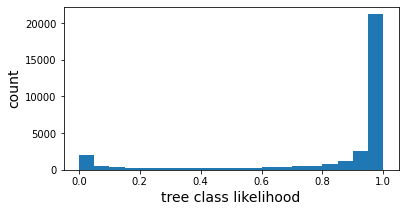
\includegraphics[width=.8\linewidth]{"./fig_histTreeClassFilter.png"}
  \caption{\label{fig:hist_tree_class} Histogram of tree class likelihoods}
\end{figure}


Details of my final tree species dataset are presented in Table \ref{tab:dataset_final} by tree species and image source.

\begin{table}[!htbp]
  \begin{center}
    \small
  \begin{tabular}{|l|r|r|r|r|}
  \hline
  Species (N) & Total & Bing & Arb. Day & Harvard \\
  \hline\hline
  Black Locust & 3587 & 3325 & 0 & 262\\
   Black Walnut & 3845 & 3327 & 23 & 495\\
   Honey Locust & 2925 & 2925 & 0 & 0\\
   Loblolly Pine & 3106 & 3059 & 47 & 0\\
   North. Red Oak & 3535 & 3236 & 42 & 257\\
   Pecan & 3875 & 3754 & 42 & 79\\
   Chinese Chestnut & 4071 & 2905 & 17 & 149\\
   \hline\hline
   Total & 24944 & 22531 & 171 & 2242\\
  \hline
  \end{tabular}
  \end{center}
  \caption{\label{tab:dataset_final} Final tree species image dataset}
  \end{table}

%------------------------------------------------------------------------
\section{Results and discussion}
\label{sec:results}
In this section I discuss my results. I start with an evaluation of the models described above and my final model selection. I then proceed with an evaluation of my selected model on my withheld test dataset with both qualitative and quantitative metrics. I also include a brief description of the evaluation metrics I use for my selected model. 

\subsection{Training results and model selection}
All models I trained achieved maximum training and validation accuracy before their final training epoch. This gives me confidence that they have achieved at least local maxima, and also that I am not overfitting these models, as I find that the training accuracy does not significantly exceed validation accuracy, especially for the transfer learning models.
I find that [[MODEL]] highest validation accuracy accross my trianing regime; I select this model for my final evaluations and for future production within tree carbon quantification apps. While ViT also performs well, its storage costs is almost four times as high as the other comparably-performing models and this may pose a limitation in the mobile app setting. My results are presented in Table \ref{tab:model_acc}.

\begin{table}[!htbp]
  \begin{center}
    \small
  \begin{tabular}{|l|l|l|r|}
  \hline
  Model & Acc. train & Acc. val & N params\\
  \hline\hline
  Softmax & 0.233 & 0.220 & 1,053,696 \\
  SVM & 0.278 & 0.196 & 1,053,696\\
  FCN & 0.284 & 0.264 & 19,268,480\\
  CNN & 0.406 & 0.327 & 5,620,656\\
  ResNetFC & 0.571 & 0.561 & 25,557,032\\
  \textbf{ResNet} & & & \textbf{25,557,032}\\
  ConvNextFC & 0.612 & 0.608 & 28,589,128\\
  ConvNext & & & 28,589,128\\
  ViT & 0.634 & 0.615 & 86,567,656\\
  \hline
  \end{tabular}
  \end{center}
  \caption{\label{tab:model_acc} Model accuracy and storage size}
  \end{table}

\subsection{Final model evaluation}
\subsubsection{Evaluation metrics}
Top-K accuracy scores refer to the percent of images for which the correct class was within the top K predicted scores. As my classifier only considers the seven common species of trees in agroforestry, I only consider small Ks, specifically Top-1 and Top-2 accuracy.

Precision, recall, and the F1 score provide alternative methods of evaluating the predictive power of a model, capturing the relationship between the true positives, false positives, and false negatives produced by a model. They are defined as follows
\begin{align*}
  \textrm{Precision} &= \frac{TP}{TP + FP}\\
  \textrm{Recall} &= \frac{TP}{TP + FN}\\
  \textrm{F1} &= \frac{2 * \textrm{Precision} * \textrm{Recall}}{\textrm{Precision} + \textrm{Recall}}
\end{align*}
I report these scores for each class, and also consider the weighted average scores across all classes. A helpful way to visualize the components of these scores is with a confusion matrix. In a confusion matrix, each row of the matrix represents the instances in an actual class while each column represents the instances in a predicted class

Lastly, I implement methods developed by Simonyan et al \cite{simonyan} to qualitatively visualize each of my classes as represented by the model. I do so for each class through gradient \textit{ascent}, generate an image that the network will recognize as the target class. This process follows the following optimization
\begin{align*}
  I^* = \arg\max_I(s_y(I) - R(I))
\end{align*}
where $s_y(I)$ is the score from a deep learning model for image $I$ and $R(I)$ is a regularizer (e.g., $\lambda \mid\mid I \mid\mid_2^2$).

\subsubsection{Quantitative evaluation results}
I now present the evaluation metrics for [[MODEL]], the final model I select through this research. [[mODEL]] achieves a XXXX Top-1 accuracy and a XXXX Top-2 accuracy. In a field setting, this implies that farmers using this tooling could identify their photographed trees XX out of 100 times, and could narrow their choice to two tree species XX out of 100 times. 

Next, I consider the results of class-wise precision and recall scores, presented in Table \ref{tab:recall}. Here I observe FINDINGS. I also evaluate the results of a confusion matrix for these predictions in Table \ref{tab:confusion}. Here I observe that [[MODEL]] is most effective at identifying [[species]] and least at identifying [[species]]. 

\begin{table}[!htbp]
  \begin{center}
    \small
    \begin{tabular}{lrrrrrrr}
      \toprule
      {} &     BL &     BW &      C &     HL &     LP &      O &      P \\
      \midrule
      BL &  71.43 &  14.29 &   0.00 &  14.29 &   0.00 &   0.00 &   0.00 \\
      BW &  25.00 &  62.50 &   0.00 &   0.00 &  12.50 &   0.00 &   0.00 \\
      C  &   0.00 &  28.57 &  57.14 &   0.00 &  14.29 &   0.00 &   0.00 \\
      HL &  16.67 &  33.33 &   0.00 &  33.33 &   0.00 &   0.00 &  16.67 \\
      LP &   0.00 &  14.29 &   0.00 &   0.00 &  85.71 &   0.00 &   0.00 \\
      O  &  14.29 &   0.00 &  14.29 &  14.29 &   0.00 &  57.14 &   0.00 \\
      P  &  12.50 &   0.00 &  25.00 &   0.00 &   0.00 &  12.50 &  50.00 \\
      \bottomrule
      \end{tabular}
  \end{center}
  \caption{\label{tab:confusion} Confusion matrix for [[MODEL]]-predicted images from test dataset. \textbf{Abbreviations:} BL=Black Locust, BW=Black Walnut, HL=Honey Locust, LP=Loblolly Pine, O=Northern Red Oak, P=Pecan, C=Chinese Chestnut}
  \end{table}


  \begin{table}[!htbp]
    \begin{center}
      \small
      \begin{tabular}{lrrrr}
        \toprule
        {} &  precision &  recall &  f1-score &  support \\
        \midrule
        BL           &      0.500 &   0.714 &     0.588 &      7.0 \\
        BW           &      0.455 &   0.625 &     0.526 &      8.0 \\
        C            &      0.571 &   0.571 &     0.571 &      7.0 \\
        HL           &      0.500 &   0.333 &     0.400 &      6.0 \\
        LP           &      0.750 &   0.857 &     0.800 &      7.0 \\
        O            &      0.800 &   0.571 &     0.667 &      7.0 \\
        P            &      0.800 &   0.500 &     0.615 &      8.0 \\
        weighted avg &      0.628 &   0.600 &     0.598 &     50.0 \\
        \bottomrule
        \end{tabular}
    \end{center}
    \caption{\label{tab:recall} Precision and recall for [[MODEL]]-predicted images from test dataset \textbf{Abbreviations:} BL=Black Locust, BW=Black Walnut, HL=Honey Locust, LP=Loblolly Pine, O=Northern Red Oak, P=Pecan, C=Chinese Chestnut}
    \end{table}

\subsubsection{Qualitative evaluation metrics}
To assist with visual interpretability and to qualitatively understand the performance of my final model, below I include images and scores of the highest-scoring images in my test dataset in Figure \ref{fig:top_imgs}, images and scores of the lowest-scoring images in my test dataset in Figure \ref{fig:bott_imgs}, and class visualizations for each class, as described above in Figure \ref{fig:class_vis}.
[[INTERPRETATION]]

\begin{figure}[!htbp]
  \centering
  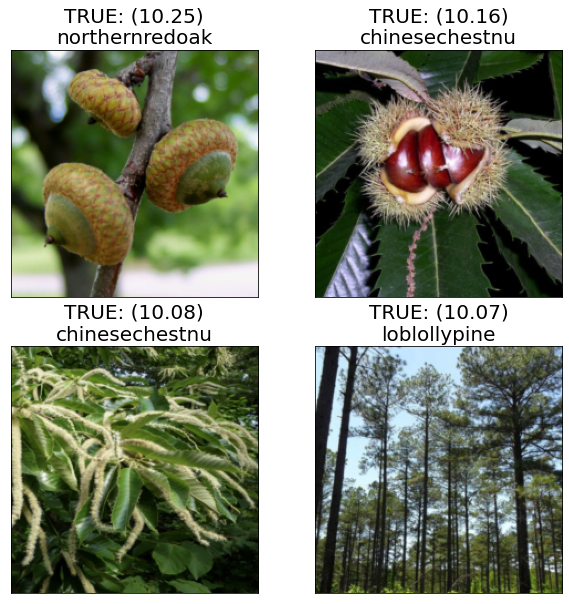
\includegraphics[width=.8\linewidth]{"./fig_top_img.png"}
  \caption{\label{fig:top_imgs} Highest scoring images in correct class}
\end{figure}

\begin{figure}[!htbp]
  \centering
  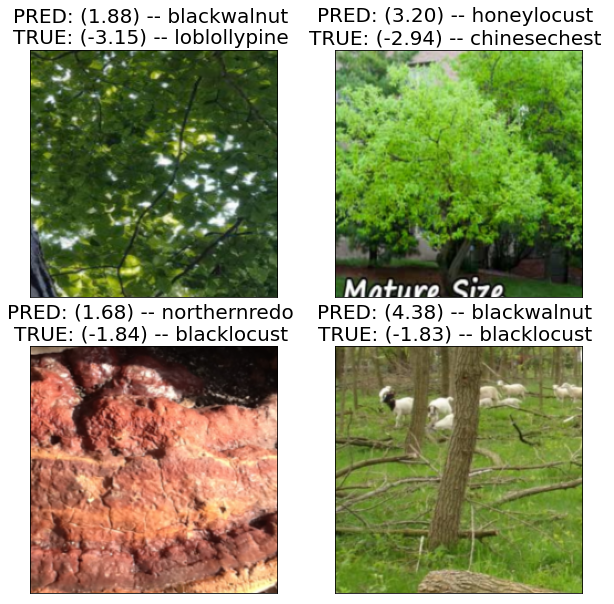
\includegraphics[width=.8\linewidth]{"./fig_bott_img.png"}
  \caption{\label{fig:bott_imgs} Lowest scoring images in correct class}
\end{figure}

\begin{figure}[!htbp]
  \centering
  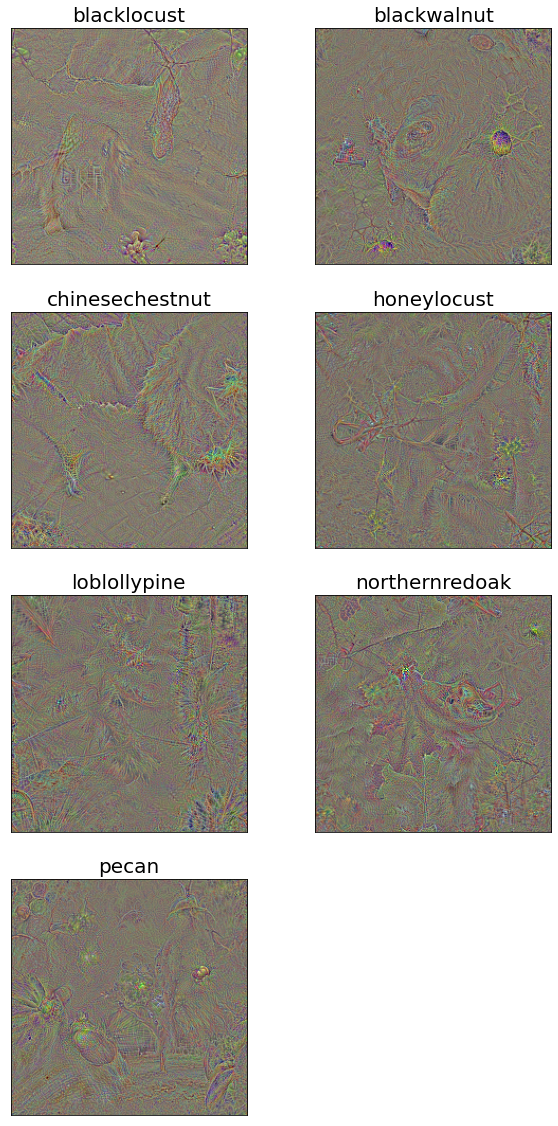
\includegraphics[width=.8\linewidth]{"./fig_class_vis.png"}
  \caption{\label{fig:class_vis} Synthetic visualizations for each class}
\end{figure}







%------------------------------------------------------------------------
\section{Conclusion and future work}
\label{sec:conclusion}
Tree species identification can integrate with a broader suite of tools to improve the accuracty of forest carbon estimation while also reducing costs. In this paper I train a tree species classifier to support carbon measurements in the agroforestry setting. I compile a novel dataset of over 24k labeled tree images and evaluate six transfer learning models for highest performance. My dataset is constructed from scraped web images, which I augment with vertical reflections and random croppings of each image and finally filtered with a binary classification model trained to detect trees.
  
I achieve a Top-1 accuracy of [[XX]] on held-out data by applying transfer learning to the [[XX]] model, training the entire last convolutional block of the model. I find this model to be better optimized for mobile-based tree species identification than other models because of its lower model parameter count. I find this final model performs best at detecting [[TREESPECIES]] with a precision and recall of XXX, respectively; it performs least well at detecting [[TREESPECIES]] with a precision and recall of XXX respectively.

As next steps in the near-term, I intend to supplement my dataset with higher fidelity images, which will come from the app that will be using the tree species classifier on agroforestry operations. As the majority of my training data comes from image searches on the internet, I suspect that increasing the share of higher quality images will likely improve Top-1 accuracy of my models. I also plan to apply the transfer learning techniques developed above on larger models like ResNet-152 and to retrain more of the convolutional or encoder layers of the model. I was able to achieve nearly a 20 percentage point increase in Top-1 accuracy for ResNet by retraining one layer deeper into the model and would like to explore how much more performance I could achieve by going deeper still. 


%------------------------------------------------------------------------
\section{Contributions and acknowledgements}
\label{sec:contrib}
This research is solo authored by Erich Trieschman and conducted entirely within the context of the Stanford course CS231N taken in the Spring Quarter of 2022. I leverage a few utility functions from homework assignments from this class as well as from tutorials provided by Pytorch \cite{PyTorch}.

All of my code, results, and the final pretrained model are available in a project repo on my GitHub, available at \url{https://github.com/etrieschman/tree-finder}

%%%%%%%%% REFERENCES
{\small
\bibliographystyle{ieee}
\bibliography{egbib}
}

\end{document}
